  


\begin{comment}
%%%%%%%%%%%%%%%%%%%%%%%%%%%%%%%%%%%
\begin{figure*}[t!]
\begin{subfigure}[htb]{0.42\linewidth}
  \centering
  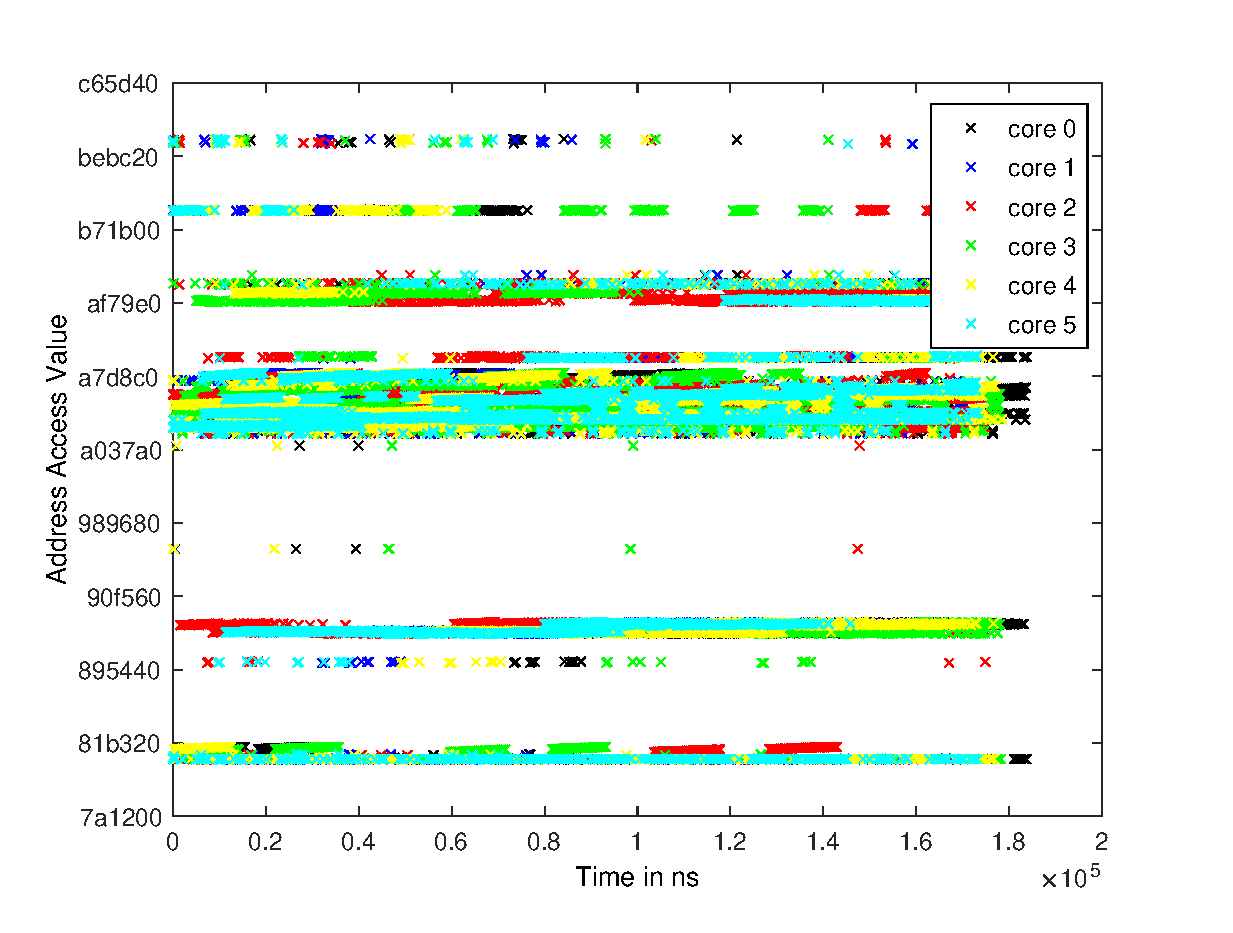
\includegraphics[height=\textwidth]{figures/add-access-soc1.eps} 
  \caption{This is a address access trace taken from a real multi-core SoC system that shows the performance of the data memory access pattern while it is executing commands. Access patterns are bulky in general.}
  \label{fig:dynamic_coding1}
\end{subfigure}
\hspace*{\fill}
\begin{subfigure}[htb]{0.42\linewidth}
  \centering
  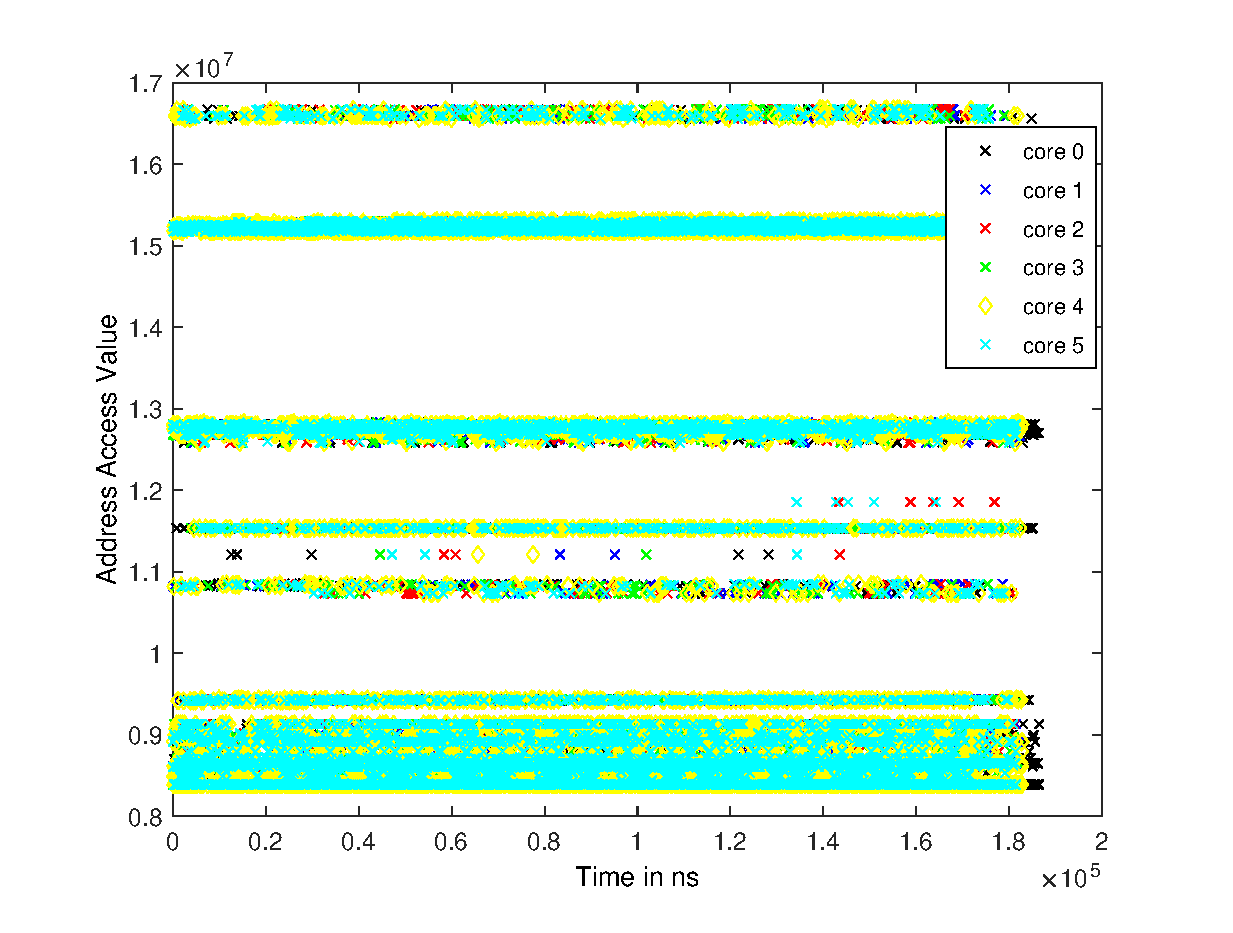
\includegraphics[height=\textwidth]{figures/add-access-soc2.eps} 
  \caption{This is an accesss pattern from another SoC system showing a multi-core access. The accesses here is more concentrated on smaller memory regions where the proposed scheme in this paper can help spread out the access resulting in higher latency. }
  \label{fig:dynamic_coding2}
\end{subfigure}
\caption{Illustration of the locality in memory access patterns using two real-life traces.}
\label{fig:dynamic_coding}
\end{figure*}
%%%%%%%%%%%%%%%%%%%%%%%%%%%%%%%%%%%%%%


\subsubsection{Dynamic coding}
\Ethan{Remove entire subsection?}
The contention in memory accesses from various cores occurs mostly when the access are to shared memory, especially when they are localized to certain memory regions. We explore the locality of the memory access over a period of time to reduce the memory overhead for storing the codes. In a multi-core system, when various cores try to work from a shared memory location, they tend to generate accesses to a localized region of memory. This motivates the idea of coding the localized region during the period of heavy access, and dynamically changing the region whenever there is change in the locality of memory accesses.

Figure \ref{fig:dynamic_coding1} shows the access pattern of a wireless SoC cores $0$ to $6$. The $y$-axis of the figure shows the address accessed by the first set of wireless SoC cores over a period of time. The $x$-axis denotes the time in nanoseconds. This plot shows that most of the access from various cores are limited to the memory range from \texttt{0x007a1200} to \texttt{0x00c65d40} (lower and higher range on the $y$-axis). It also suggests that most (about 60\%) of the accesses belong to the memory region of \texttt{0x00a037a0} to \texttt{0x00b71b00}. We make similar observation from Figure \ref{fig:dynamic_coding2} for another set of traces with highly concentrated, spottier access patterns. Here again, all of the access for a duration of approximately 0.2 ms is in the address range of \texttt{0x007a1200} to \texttt{0x01036640}.

From the above observations, we demonstrate the idea of coding the highly accessed portion of the memory. This scheme benefits from a huge reduction of the memory overhead with coding. The reduction the memory overhead can be used to reduce the complexity of the decoder by using simple coding functions (e.g. XOR) and for densely coding (e.g. repeatedly coding a single element using 2 elements). 
The scheme of dynamic coding requires that the currently coded region changes when the access pattern changes. That is, the localized memory area that is most heavily accessed can change, and it will require the system to recode the new localized access region. We assume that the working area of a program changes with change in the input parameters to the program. It can be easily observed from the above figures that the working area or the localized area is constant for at least $0.2$ ms\Ankit{Is $0.2$ ms long enough?}. This suggests that the switching of the coded region is not very frequent. During these periods of coding switches, it is also guaranteed that the number of accesses served from the memory is at worst equal to the number of banks available. In other words, coding the memory has no performance degradation compared to non-coding during these times. 

The system also needs to maintain an algorithm to observe the access pattern of the cores, and make a decision when it is time to code a new memory region. To do this, the memory controller tracks the most accessible region during a time period and makes a decision to slide/shift the coded region. This shift in the coded region requires the update of the parity bank for the new region. This process is carried out in conjunction with the ongoing access to the newly coded region. Therefore, this operation only requires writes to the parity banks, since we can use the current reads from the coded region to access the data that is to be coded. In addition, reads are also scheduled in the idle periods, when there is no read or write request to the bank/banks.


Dynamic coding requires the system to divide the memory into subregions and to keep track of accesses in these sub-regions. Once the number of accesses to a sub-region reaches a given threshold, it must then make this region the currently coded area. We propose this mechanism based on window concept. The system maintains a tuple of sub-regions such as [Starting Address, Length]. Each sub-region is thus given a starting address and length. Any access to a particular sub-region is considered as a hit. The system has a hit counter associated with each of the sub-region which is incremented for each hit. The system makes a decision of coding a particular sub-region based on its counter value. The number of coded sub-regions at a particular time is based on the sub-region size and the code storage size. The eviction of a coded region follows the LRU policy similar to cache.


%%%%%%%%%%%%%%%%%%%%%%%%%%%%%%%%%%%
\begin{figure*}[htb] \centering
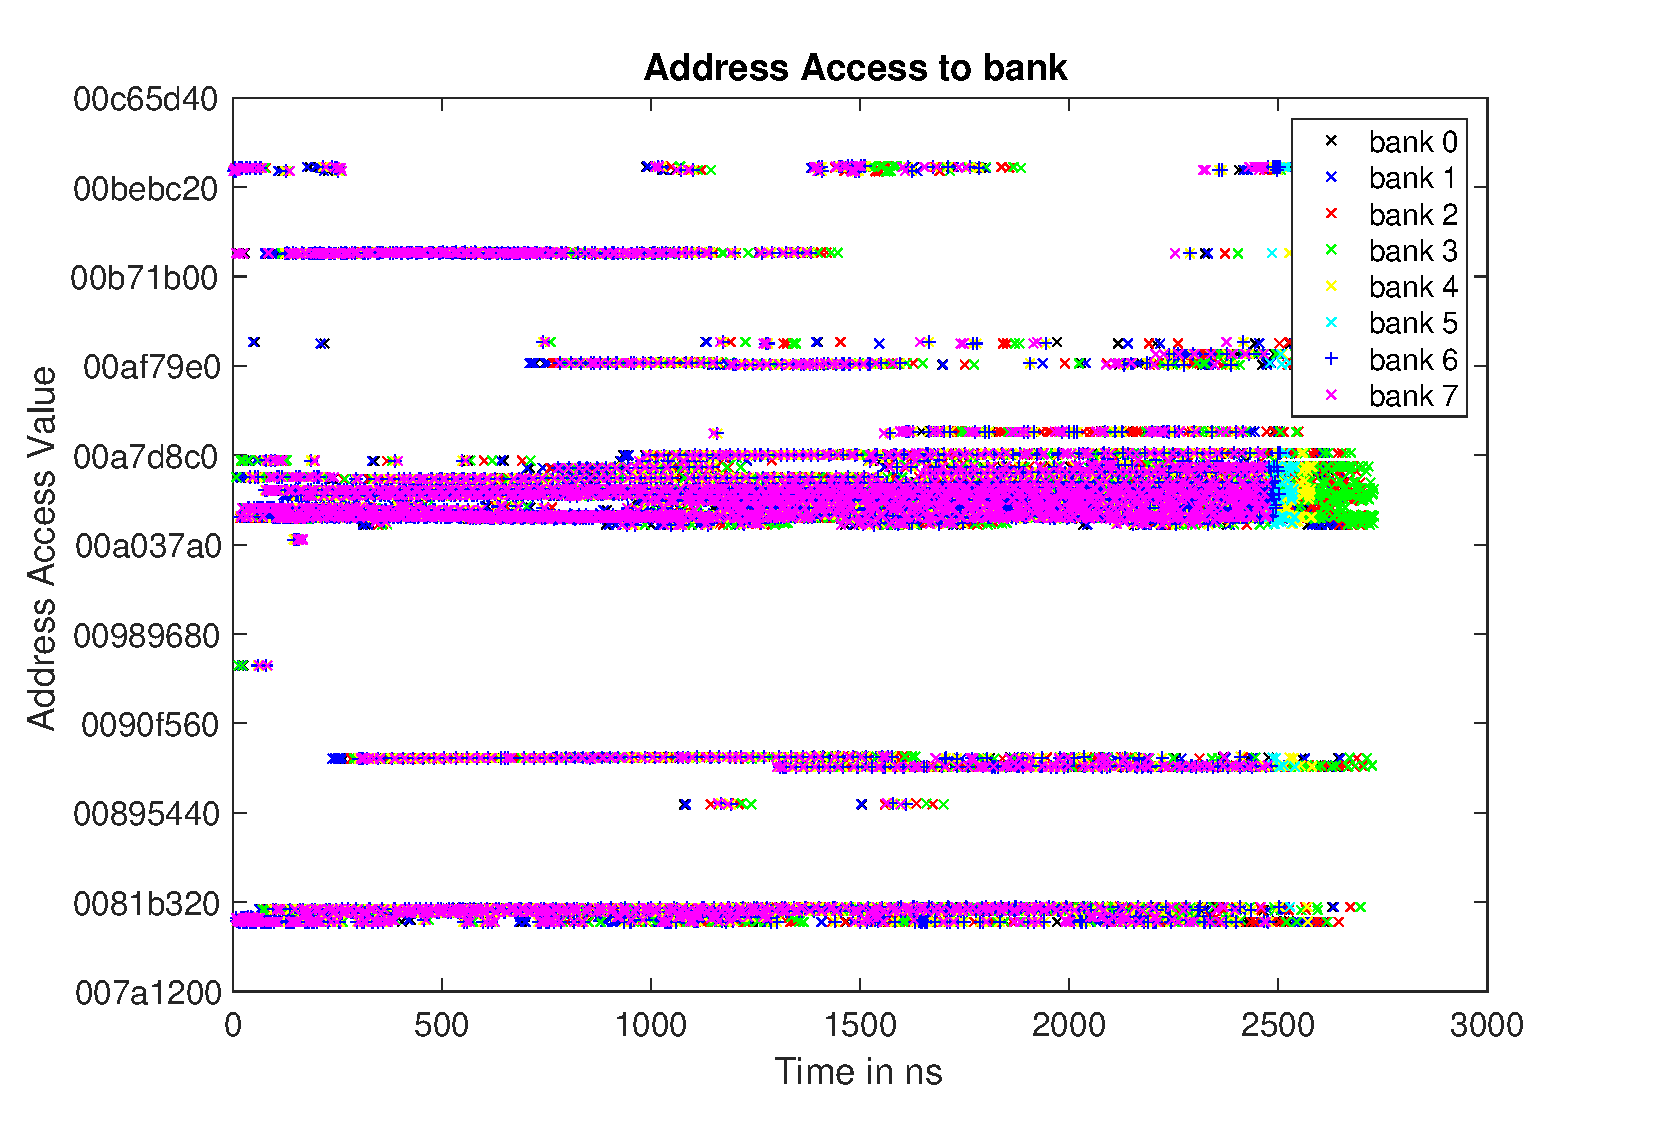
\includegraphics[width=0.48\linewidth]{figures/prefetch1.eps} 
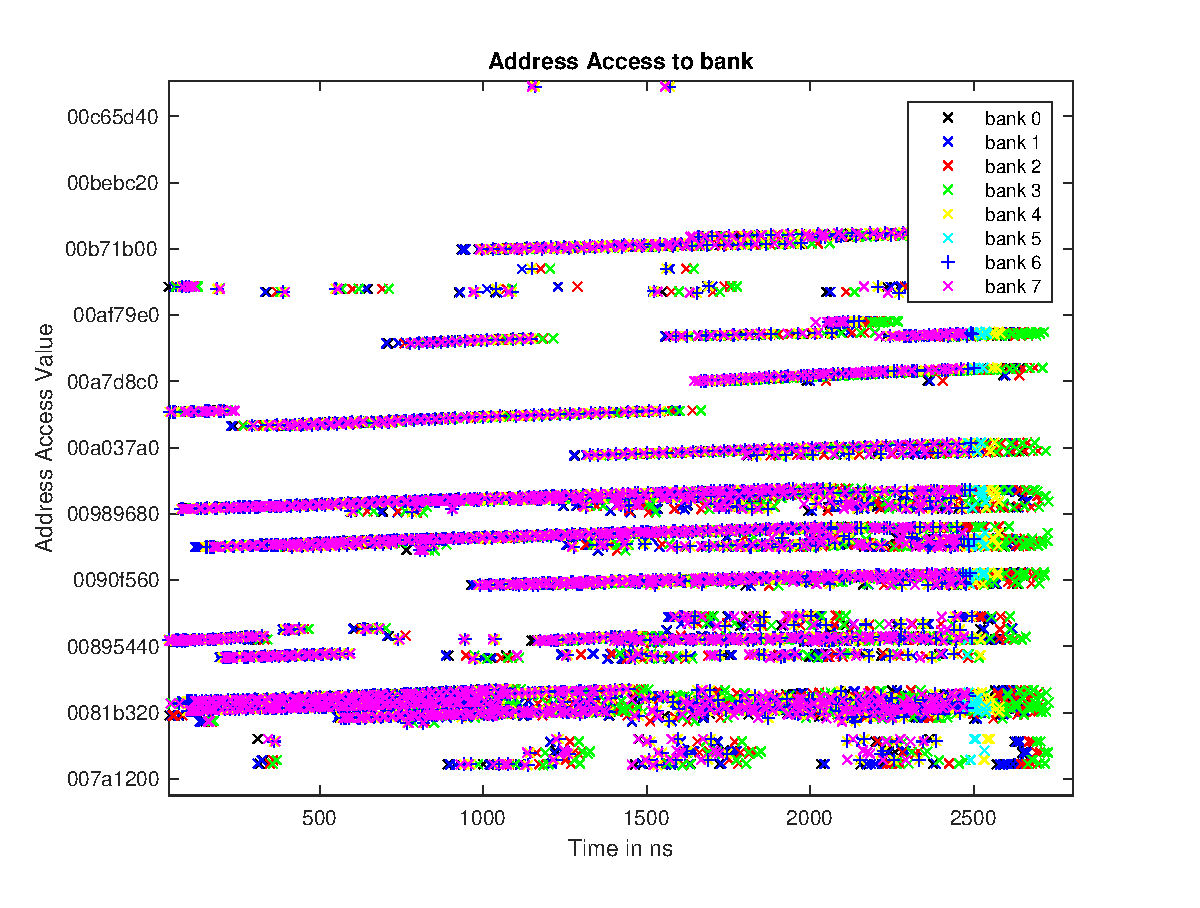
\includegraphics[width=0.48\linewidth]{figures/prefetch2.eps} 
\caption{memory accesses to a bank with respect to time}
\label{fig:prefetch1}
\end{figure*}
%%%%%%%%%%%%%%%%%%%%%%%%%%%%%%%%%%%

\subsubsection{Prefetching codes}
\Ethan{Remove entire subsection?}
The technique of dynamic coding reduces the memory overhead by exploiting the localized nature of memory accesses from the cores. In this subsection, we explore prefetching the coded data to reduce the access overhead and contention caused for fetching the codes. This is done by using the gaps in the memory access to any bank and using these gaps to prefetch the code/data for a future memory access. During a program, there are access cycles when certain banks do not have any access scheduled for a read/write. We propose the prefetching technique where we look forward in the queue and anticipate a prefetch for the data/code for that bank. We explore the implementation of a memory prefetching unit, similar to an instruction or cache prefetching unit. This unit can detect linear access patterns to regions in memory.  For example, if a string of memory accesses are issued in sequential byte sized order, then the prefetching unit will predict the next access to be in byte increments. The memory prefetching works by fetching a predicted address from the parity bank during accesses that the parity bank is idle. When future memory accesses are issued, they are first checked with the prefetched data to see if they can be used to decode any subsequent accesses memory accesses. If so, the memory access is obtained from the current accesses and prefetched data. 

For example, say the prefetcher sees 2 consecutive memory requests in a row. It then predicts that the next two accesses, locations $a_0$ and $b_0$, are likely to be accessed in the near future. It reads $a_0 + b_0$ from the parity bank for future use. Next, access to location $a_0$ and $b_0$ are issued to the memory. Now, instead of reading both $a_0$ and $b_0$, only a single location has to be read from in memory, while the other location can be obtained from the prefetched data. This allows for an additional access to be issued from the now free memory bank.  In these cases, it is possible to obtain up to two additional memory accesses in a given cycle, one from the prefetched data and one from the parity bank.

Implementation of a memory prefetch should only require overhead for space and the associated logic to implement it. Since memory accesses are often stalled due to bank conflicts, checking pending accesses to the prefetched data should require no additional time overhead. As memory accesses wait to be issued in the bank queues, they can simultaneously be checked with the prefetched data. Thus, no extra latency is anticipated by the addition of a memory prefetching unit.

Figure~\ref{fig:prefetch1} shows two plots of memory accesses to a bank with respect to time. The left figure shows the accesses to the memory bank by various cores. The right side figure shows a zoomed view of the accesses in the dense access region. This figure suggests the linearity of accesses. The system can look ahead in the queue to detect the consecutive address request for a memory bank and schedule a prefetch of the associated code. In Figure~\ref{fig:prefetch2}, we simulate the prefetching of the code by using a window of length $100$. That is, we look ahead to $100$ request in the queue and find out the occurrence of consecutive address in the window. The plot suggest high occurrence of the consecutive addresses in the bank which can be served by prefetching the codes. 
\end{comment}